\chapter{Holographic Particle Characterization}
\label{ch:hvm}

\newcommand{\einc}{\vec{E}_{\text{inc}}}
\newcommand{\escat}{\vec{E}_{\text{s}}}
\newcommand{\eadd}{\vec{E}_{\text{add}}}

\section{Overview}

Holographic particle characterization (HPC) uses coherent
illumination to measure properties of micrometer-sized particles,
primarily their size, refractive index, and three-dimensional position.
Coherent imaging preserves the phase information that is averaged-away
in conventional incoherent image. The physical properties of individual
scatterers are encoded in this phase information and can be extracted by fitting
the resulting intensity patterns to an appropriate light scattering theory.
For non-absorbing dielectric spheres with a diameter between $\num{1}$ and $\SI{10}{\um}$,
this technique yields nanometer-scale precision for the three-dimensional
position and radius, and part-per-thousand precision for the refractive
index\cite{krishnatreya14}.

In this chapter, we acquaint the reader with our primary experimental
HPC setup and in so doing outline the salient physical processes underlying
the technique. We then describe the Lorenz-Mie theory of light
scattering that provides the basis for our analytical technique,
discuss our implementation of image analysis, and 
conclude with a number of applications of holographic particle
characterization.

\section{Experimental Setup}
\label{ch:hvm:sec:hvm}

Fig.~\ref{fig:hvm_setup} presents our custom-built in-line holographic
microscope. Our setup illuminates the sample plane with a blue
($\SI{447}{nm}$ vacuum wavelength), linearly polarized laser beam
(Coherent Cube). The axis of polarization is aligned to within
\SI{1}{\degree} of the horizontal axis of the camera. 
The beam's $\SI{25}{\mW}$ of power is spread over
the $\SI{3}{\mm}$ beam diameter, producing an average irradiance
of $\SI{0.88}{\mW / \mm^2}$. Before illuminating the sample, the beam
passes through a quarter-wave plate and a polarizing beam splitter
(ThorLabs CCM1-PBS251) to optimize the beam's linear polarization, to
enable beam attenuation and to provide an optical pathway for
optional bright-field illumination.


\begin{figure}
  \centering
  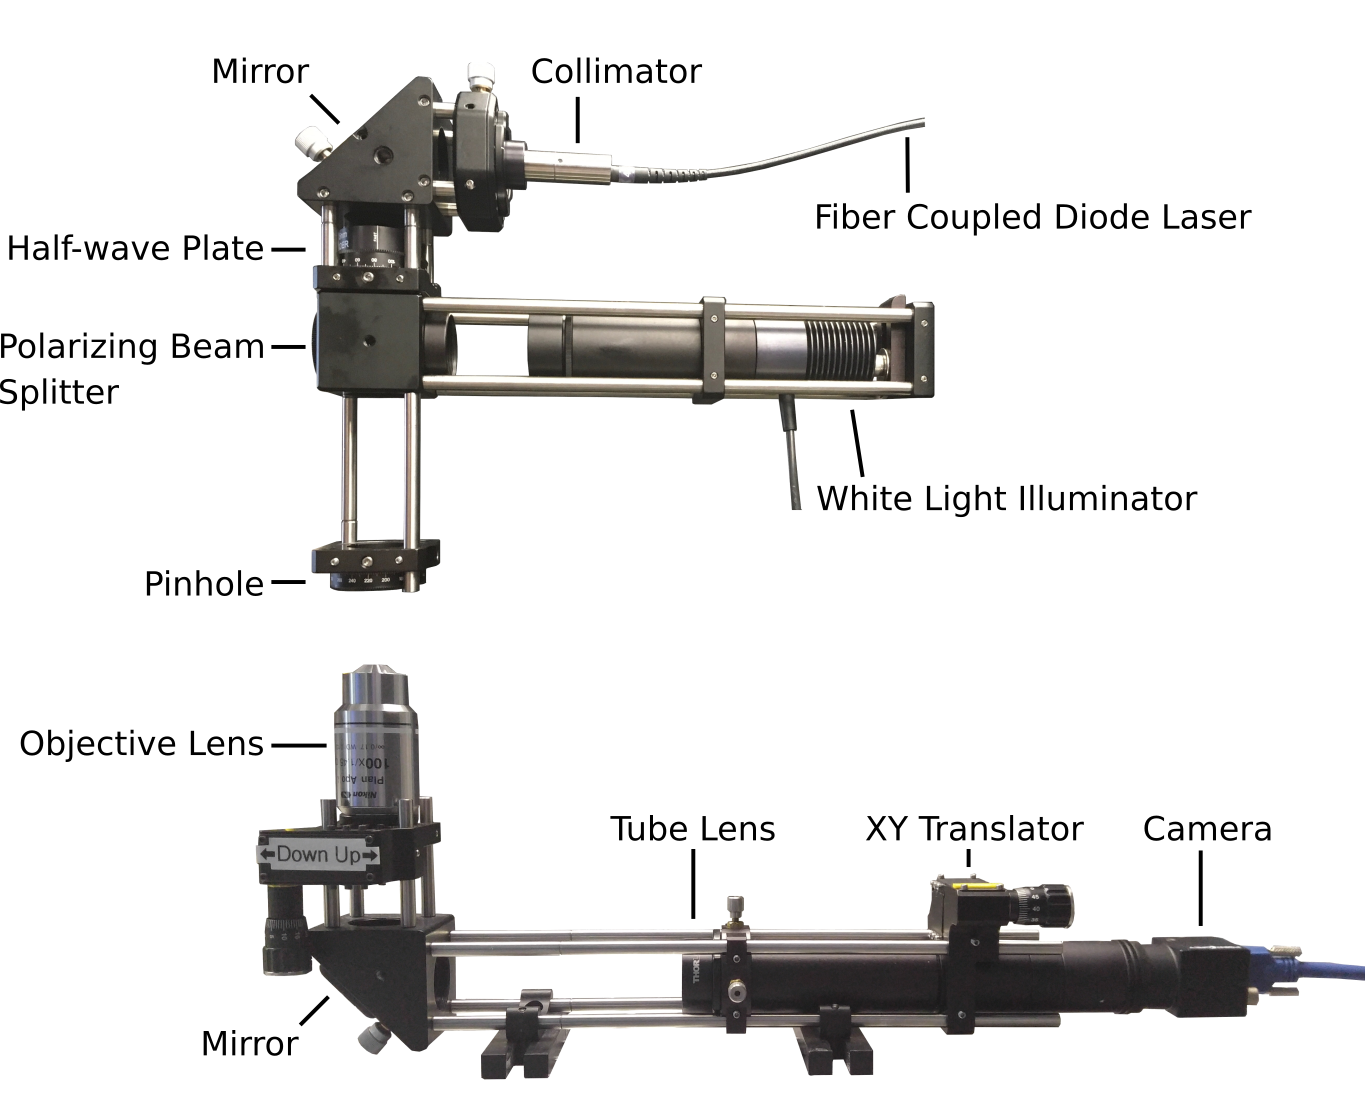
\includegraphics[width=0.75\columnwidth]{hvm_setup.png}
  \caption{A schematic of an inline holographic video microscope.}
  \label{fig:hvm_setup}
\end{figure}


The coherent illumination and the light scattered by the sample are collected by a
standard microscope objective (Nikon Plan Apo, $\num{100}\times$,
numerical aperture $\num{1.45}$, oil immersion) and then focused
by a $\SI{200}{\mm}$ tube lens onto a grayscale CCD camera
(NEC TI-324AII).
The camera's output is either directed to a DVR (Pioneer 520HS) that records
it as uncompressed digital video or else is digitized directly (Sensoarray 22555)
to $\SI{8}{bits\per pixel}$ and at $\SI{29.98}{frames\per\sec}$ and is relayed
directly to a computer workstation.
%The digital camera digitizes the resulting intensity
%pattern to $8$-bits per pixel at $\SI{29.97}{frames / \sec}$ and relays the
%resulting array of data to either a DVR (Pioneer 520HS) to record
%on a DVD or directly to the hard disk of a personal computer.
Each pixel in the camera's $\si{640\times 480}$ array of pixels has a width of
$\SI{13.5}{\um}$. After $100\times$ magnification, a pixel in the
image has an effective size of $\SI{0.135}{\um}$.

Each recorded image documents the interference between the incident
electric field and the resulting scattered waves. By fitting
to a model based on the theory of light scattering, we will measure the physical
properties of the scatterers contributing to the scattered field
at the focal plane of the objective.

% Description of trapping?


  % BLURB connecting HPC to DHM
%Holographic particle characterization is one of several
%digital holographic microscopy (DHM) techniques.
%DHM differs from traditional bright-field microscopy
%by preserving, collecting, and making quantitative use of phase
%information. In most variants of DHM, each recorded
%wavefront can be numerically reconstructed, or rather
%{\it un}-propagated, all the way back to a scattering event
%to produce an image of the scatterer. By reconstructing
%several planes around the scatterer, each hologram
%can provide insight into the topography of each scatter
%in the field of view.

%Holographic particle characterization differs from DHM by analytically
%fitting the scatter's properties to the resulting

\begin{figure}
  \centering
  \includegraphics[width=\textwidth]{hvm_image_formation}
  \caption{A time series depicting the image formation process. (a) The incident
    electric field propagates in the $+\hat{z}$ direction. (b) The
    incident field passes through a spherical scatterer causing a
    spherically expanding scattered wave in response. (c) The incident
    field and the scattered field combine at the focal plane to produce
    an image.}
  \label{fig:image_formation}
\end{figure}


\subsection{Image formation}
\label{ch:hvm:sec:hvm:ssec:overview}

The image formation process at the focal plane of the objective
is depicted in Fig.~\ref{fig:image_formation}. Fig.~\ref{fig:image_formation}(a)
shows the coherent illumination, or incident field $\einc (\vec{r})$, propagating in the $+\hat{z}$ direction
through the sample and toward the focal plane of the objective. We model the incident field
as a plane wave polarized in the $\hat{x}$ direction, 
\begin{equation}
  \label{eq:incidentfield}
  \einc(\vec{r}) = E_0\,  e^{i \varphi_0(\vec{r})} \, e^{i kz} \, \hat{x},
\end{equation}
with magnitude $E_0$, phase profile $\varphi_0(\vec{r})$, and wavenumber
$k = 2\pi n_m/\lambda$ in a medium of refractive index, $n_m$.
Monochromatic light has a time dependence of $e^{-i \omega t}$. Measurements of
the light's intensity are time averaged over the duration of the camera's exposure
period of at least $\SI{10}{\us}$. As we will be imaging with $\SI{447}{nm}$ blue
light ($\omega \approx \SI{670}{THz}$), our time average will include
nearly \num{7} billion full cycles. We will therefore safely neglect this time
dependence.


\begin{figure}
  \centering
  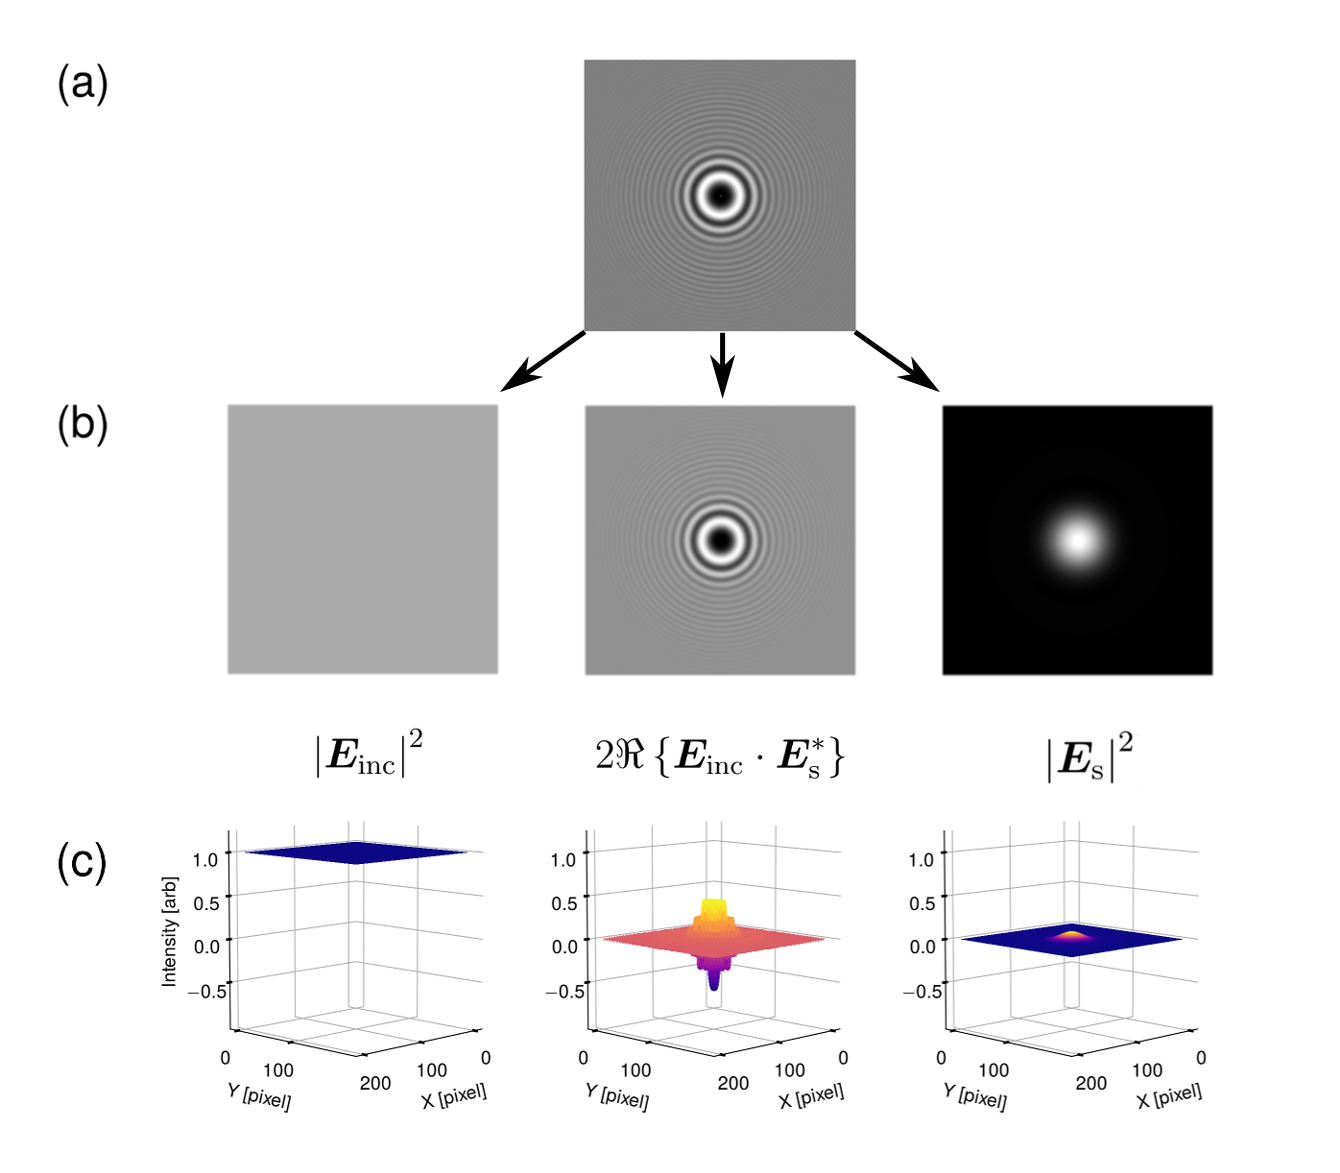
\includegraphics[width=\textwidth]{hvm_three_contributions}
  \caption{Depicting the three contributions to a holographic image. (a) The
    resulting intensity from a micrometer-sized scatterer above the focal plane.
    (b) The three contributions shown separately. (c) The magnitude of intensity
  for each term normalized by the intensity of the incident field.}
  \label{fig:three_contributions}
\end{figure}

As the incident illumination propagates freely through the sample, scatterers
whose refractive index differs from the medium's will emit a diverging scattered wave,
$\escat(\vec{r})$, in response. Fig.~\ref{fig:image_formation}(b) depicts the incident
field and resulting scattered field propagating toward the focal plane.
For the scatterers of interest in this study, the scattered field is dominated by
forward scattering and the scatterer absorbs a negligible proportion of the
incident wave.

The incident field and scattered field continue propagating and eventually pass through
the focal plane, as depicted in Fig.~\ref{fig:image_formation}(c). The intensity of the image
formed in the focal plane can be described as
\newcommand{\preint}{\frac{n_mc\epsilon_0}{2}}
\begin{align}
  I(\vec{r}) &= \preint\abs{\einc + \escat}^2\\
    &= \preint\left ( \abs{\einc}^2 + \einc\cdot\escat^* + \einc^*\cdot\escat + \abs{\escat}^2 \right ) \\
    &= \preint\left (\abs{\einc}^2 + 2\Re\left \{\einc\cdot\escat^*\right \} + \abs{\escat}^2 \right ) \label{eq:image_formation}
\end{align}
where $c$ is the speed of light in a vacuum, and $\epsilon_0$ is the vacuum permittivity.
We assumed here that the medium is non-magnetic ($\mu_r=1$).

The relative contributions of the terms in Eq.~\eqref{eq:image_formation}
are illustrated in Fig.~\ref{fig:three_contributions} for a $\SI{1.0}{\um}$ diameter
polystyrene sphere ($n = 1.59$) a distance of $\SI{12}{\um}$ above the imaging plane
with pixel size $\SI{0.135}{\um}$.
The first term, $\abs{\einc}^2$, is constant over the field of view and
incorporates no phase information. The third term,
$\abs{\escat(\vec{r})}^2$, is also real-valued but is not constant over the field of view.
The second term, $2\Re\left \{\einc\cdot\escat^*(\vec{r})\right \}$, contributes the
spatially-varying interference pattern from the phase profile of the scattered wave.
% Discussion of DC terms? Does DC Stand for duty cycle?
% Pull out E_0?
% Discuss relative sizes of terms.

\subsection{Scattering}
\label{ch:hvm:sec:hvm:ssec:scattering}

We assume that the amplitude of the scattered wave is proportional to the
amplitude of the incident wave at the scatterer's position.
We therefore model the scattered field as
\begin{equation}
  \label{eq:gen_scattered}
  \escat(\vec{r}) = E_0(\vec{r}_p)\, \vec{f}_s \left ( k \left ( \vec{r} - \vec{r}_p \right ) \right ) ,
\end{equation}
where $E_0(\vec{r}_p)$ is the amplitude of the wave illuminating the scatterer at $\vec{r}_p$,
and $\vec{f}_s(k\vec{r})$ describes how the particle $s$ scatters $\hat{x}$-polarized light.
The scattering function $\vec{f}_s(k\vec{r})$ depends inherently on the shape, size,
and composition of the scatterer. When the scattered field is adequately described by
\eqref{eq:gen_scattered}, the image in the focal plane linearly scales with the
incident field intensity $\abs{\einc}^2$,
\begin{equation}
  \label{eq:gen_norm}
  I(\vec{r}) = \preint\abs{\einc}^2\abs{\uvec{x} + \vec{f}_s(k(\vec{r}-\vec{r}_p))}^2.
\end{equation}
This is the model we use to analyze holograms of colloidal particles.

With the exception of \autoref{ch:dimpled}, our study will focus exclusively on
spherical scatterers. The Lorenz-Mie theory offers an exact solution for $\vec{f}_s(\vec{r})$
in the case of a spherical scatterer illuminated with $\hat{x}$-polarized light.
We will provide a brief overview of the Lorenz-Mie theory to build intuition
for the scattered wave's dependence on the spherical scatter's properties; a
more comprehensive account is provided in reference \cite{bohren83}.



\subsubsection{Lorenz-Mie Theory}
\label{ch:hvm:sec:hvm:ssec:scattering:sssec:lm_theory}

\begin{figure}
  \centering
  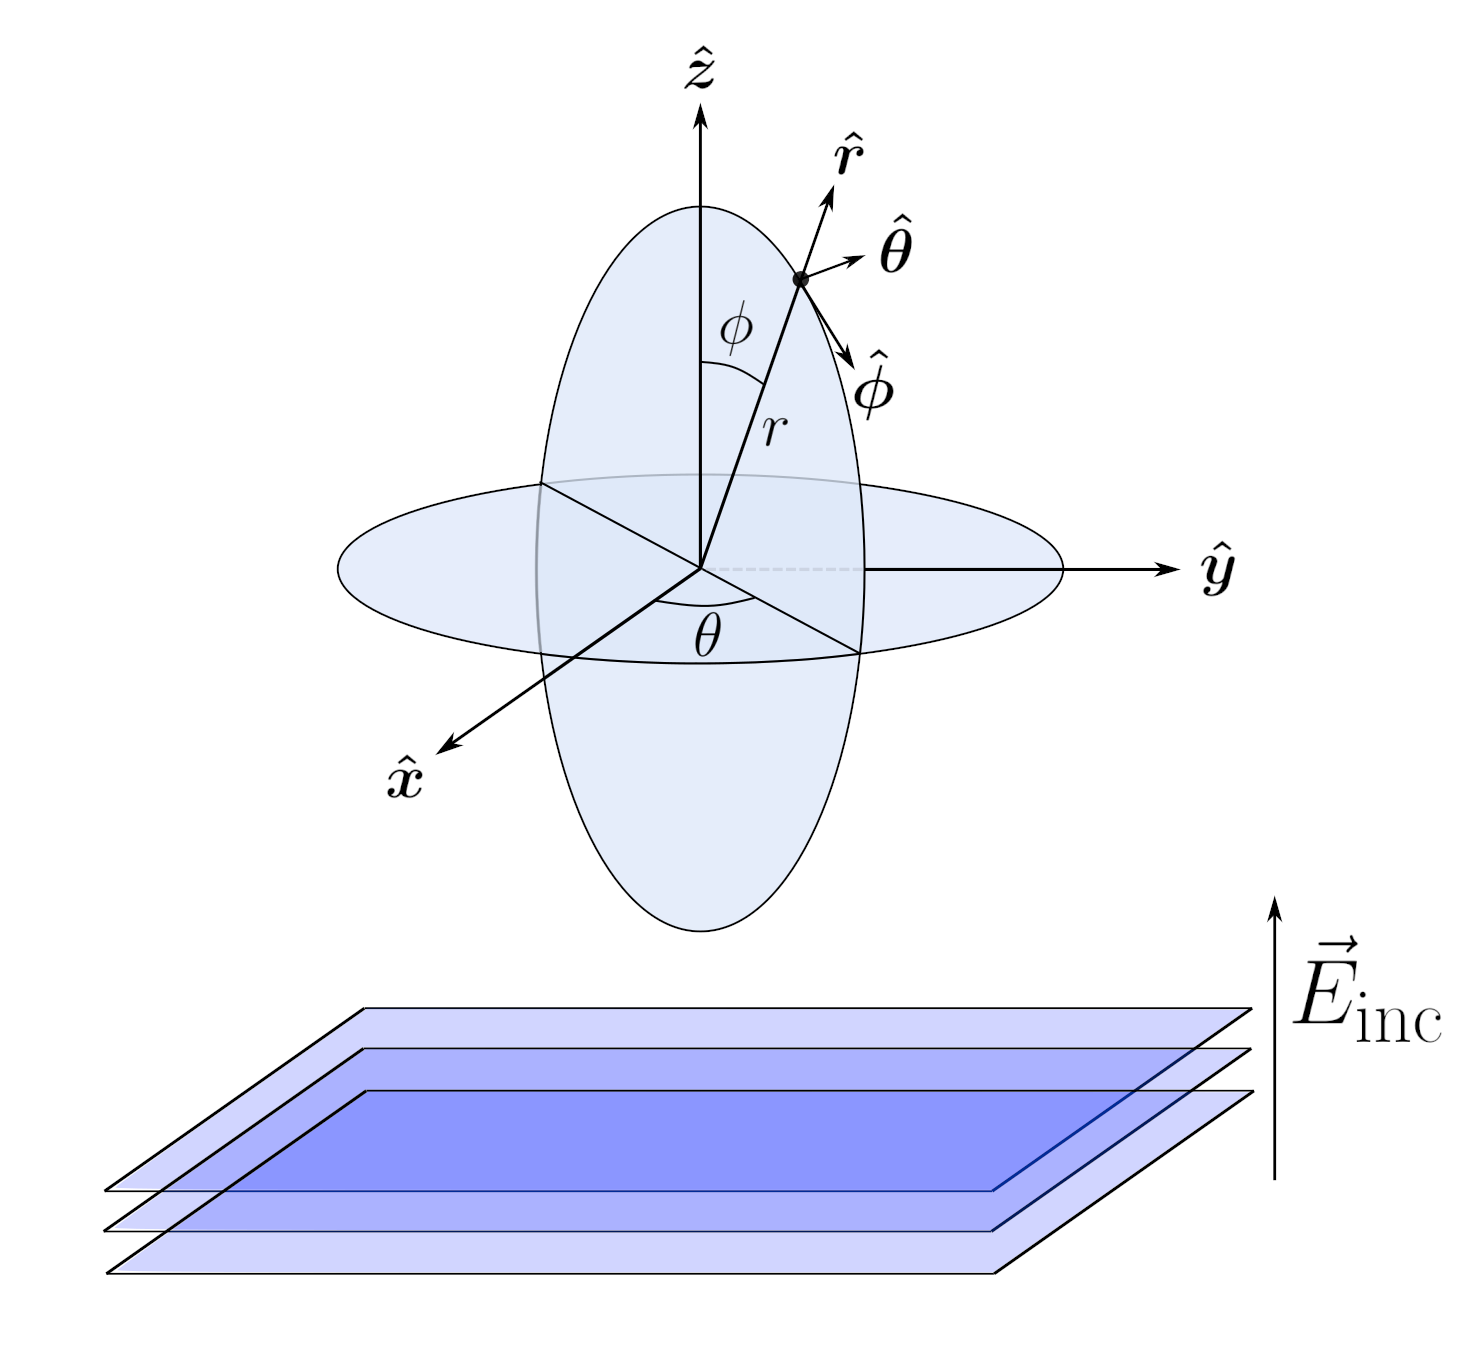
\includegraphics[width=0.5\columnwidth]{hvm_spherical_coords}
  \caption{Spherical coordinates for describing the Lorenz-Mie theory.
    The origin of the coordinate system rests at the center of the
    spherical scatterer. For viewing ease, the positive $\uvec{z}$ direction
  is depicted upwards, the opposite of Fig.~\ref{fig:image_formation}.}
  \label{fig:hvm_spherical_coords}
\end{figure}

We begin by considering a homogeneous, dielectric sphere of radius $a_p$ and refractive
index $n_p$ situated at a position $r_p$ in a medium with refractive index $n_m$.
We define a spherical coordinate system whose origin coincides with
the sphere as depicted in Fig.~\ref{fig:hvm_spherical_coords}
The incident beam is modeled as a plane wave of the form
\eqref{eq:incidentfield} which propagates toward
the scatterer from the $-\hat{z}$ direction. The scattering event
leads to three fields, namely the incident field, an external scattered
field, and an internal scattered field, all of which must match boundary conditions
at the surface of the sphere.  Based on the work of Kla\u{c}ka \emph{et al}~\cite{klacka07},
we conclude that the electrostatic
potential at the surface of a micrometer-scale sphere would have to be implausibly high
($\SI{E8}{V}$) before surface charge or current would appreciably affect the scattering
of visible light and therefore a recorded image. Therefore,
we adopt the usual assumption of a charge-free and current-free surface.

The internal and external fields in the vicinity of a sphere are most naturally
expressed as an expansion in vector spherical harmonics. Vector spherical harmonics
provide an orthonormal basis for the solutions to Maxwell's wave equations in free space.
The Lorenz-Mie solution amounts to expressing the incident plane wave as
a sum of vector spherical harmonics and matching the boundary conditions
at the surface of the spherical scatterer. After matching the boundary
conditions\cite{bohren83,mishchenko96}, the resulting external scattering function is
%The Lorenz-Mie theory
%constitutes an exact solution for a plane wave scattering off of a
%dielectric sphere in a homogeneous medium.

\begin{equation}
\label{eq:scatteredfield}
  \vec{f}_s(k \vec{r}) = \sum_{n=1}^\infty \, f_n \, \left(
    i a_n \, \vec{N}^{(3)}_{e1n}(k \vec{r}) - b_n \,
    \vec{M}^{(3)}_{o1n}(k \vec{r})
    \right),
\end{equation}
where $f_n=i^n (2n+1)/[n(n+1)]$, and $\vec{M}^{(3)}_{o1n}(k\vec{r})$ and 
$\vec{N}^{(3)}_{e1n}(k\vec{r})$ are the vector spherical harmonics,
\begin{equation}
    \vec{M}^{(3)}_{o1n}(k\vec{r}) = \frac{\cos\phi}{\sin\theta} \,
  P^1_n(\cos\theta) \, j_n(\rho) \, \uvec{\theta}
  - \sin\phi \, \frac{dP^1_n(\cos\theta)}{d\theta} \, j_n(\rho) \, \uvec{\phi},
\end{equation}
and
\begin{multline}
  \vec{N}^{(3)}_{e1n}(k\vec{r}) = n(n+1) \, \cos\phi
  \,P^1_n(\cos\theta) \, \frac{j_n(\rho)}{\rho} \, \uvec{r} \\
  + \cos\phi \, \frac{dP^1_n(\cos\theta)}{d\theta} \,
  \frac{1}{\rho} \frac{d}{d\rho}\left[ j_n(\rho)\right] \, \uvec{\theta} \\
  - \frac{\sin\phi}{\sin\theta} \, P^1_n(\cos\theta) \,
  \frac{1}{\rho}\frac{d}{d\rho}\left[\rho j_n(\rho)\right] \, \uvec{\phi}
\end{multline}
Here, $\rho = kr$ is the reduced radial coordinate,
$P^1_n(\cos\theta)$ is the associated Legendre polynomial of the
first kind, and $j_n(\rho)$ is the spherical Bessel function of the
first kind of order $n$.
The expansion coefficients $a_n$ and $b_n$ in Eq.~(\ref{eq:scatteredfield})
are given by \cite{bohren83}

\begin{equation}
  \label{eq:an}
  a_n = \frac{n_p^2 \, j_n(x_p) \left[x_m \, j_n(x_m)\right]^\prime -
    n_m^2 \, j_n(x_m) \left[x_p \, j_n(x_p)\right]^\prime}{
    n_p^2 \, j_n(x_p) \left[x_m \, h^{(1)}_n(x_m)\right]^\prime -
    n_m^2 \, h^{(1)}_n(x_m) \left[x_p \, j_n(x_p)\right]^\prime},
\end{equation}
and
\begin{equation}
\label{eq:bn}
  b_n = \frac{j_n(x_p) \left[x_m \, j_n(x_m)\right]^\prime -
    j_n(x_m) \left[x_p \, j_n(x_p)\right]^\prime}{
    j_n(x_p) \left[x_m \, h^{(1)}_n(x_m)\right]^\prime -
    h^{(1)}_n(x_m) \left[x_p \, j_n(x_p)\right]^\prime},
\end{equation}

where primes denote derivatives of function with respect to the argument
of the embedded special function, and $x_m = \frac{2\pi n_m}{\lambda} a_p$
and $x_p = \frac{2\pi n_p}{\lambda} a_p$ are the reduced particle size according
to the medium and to the particle respectively. The infinite
sum in \eqref{eq:scatteredfield} can be safely truncated after
$x_m + 4x_m^{\frac{1}{2}} + 2$ terms\cite{wiscombe80}.

A few comments help to clarify how Eqs.~\eqref{eq:gen_norm} through
\eqref{eq:bn} can be used to track and characterize colloidal particles.
The vector spherical harmonics do not depend on the scatterer's properties;
the scatterer's influence on the external scattered field is completely contained
in the coefficients.
The coefficients $a_n$ and $b_n$ converge to zero as $n_p$ approaches $n_m$, which
is the case for index-matched particles.
The condition for terminating the series in \eqref{eq:scatteredfield} depends only on
the refractive
index of the medium and the size of the particle in units of the wavelength. Given a medium
refractive index of $1.33$ and wavelength of $\SI{447}{\nm}$, the number of terms ranges
from $50$ for a $\SI{1}{\um}$ diameter sphere to more than $\num{200}$ for a
$\SI{10}{\um}$ sphere.
% Should n_p = n_m.. these computations would be a waste!


\subsection{Image Analysis}

We analyze each of our recorded images to extract information about the particles
scattering light into the field of view.  Because the scattered wave's electric
field approximately decays as $r^{-1}$, each scatterer's influence on the
resulting image is confined to a limited region of the image; we will
refer to each of these regions of interest as holographic features.  Given an experimental
image, our task will be to isolate these holographic features and fit each
to the Lorenz-Mie theory.

\begin{figure}
  \centering
  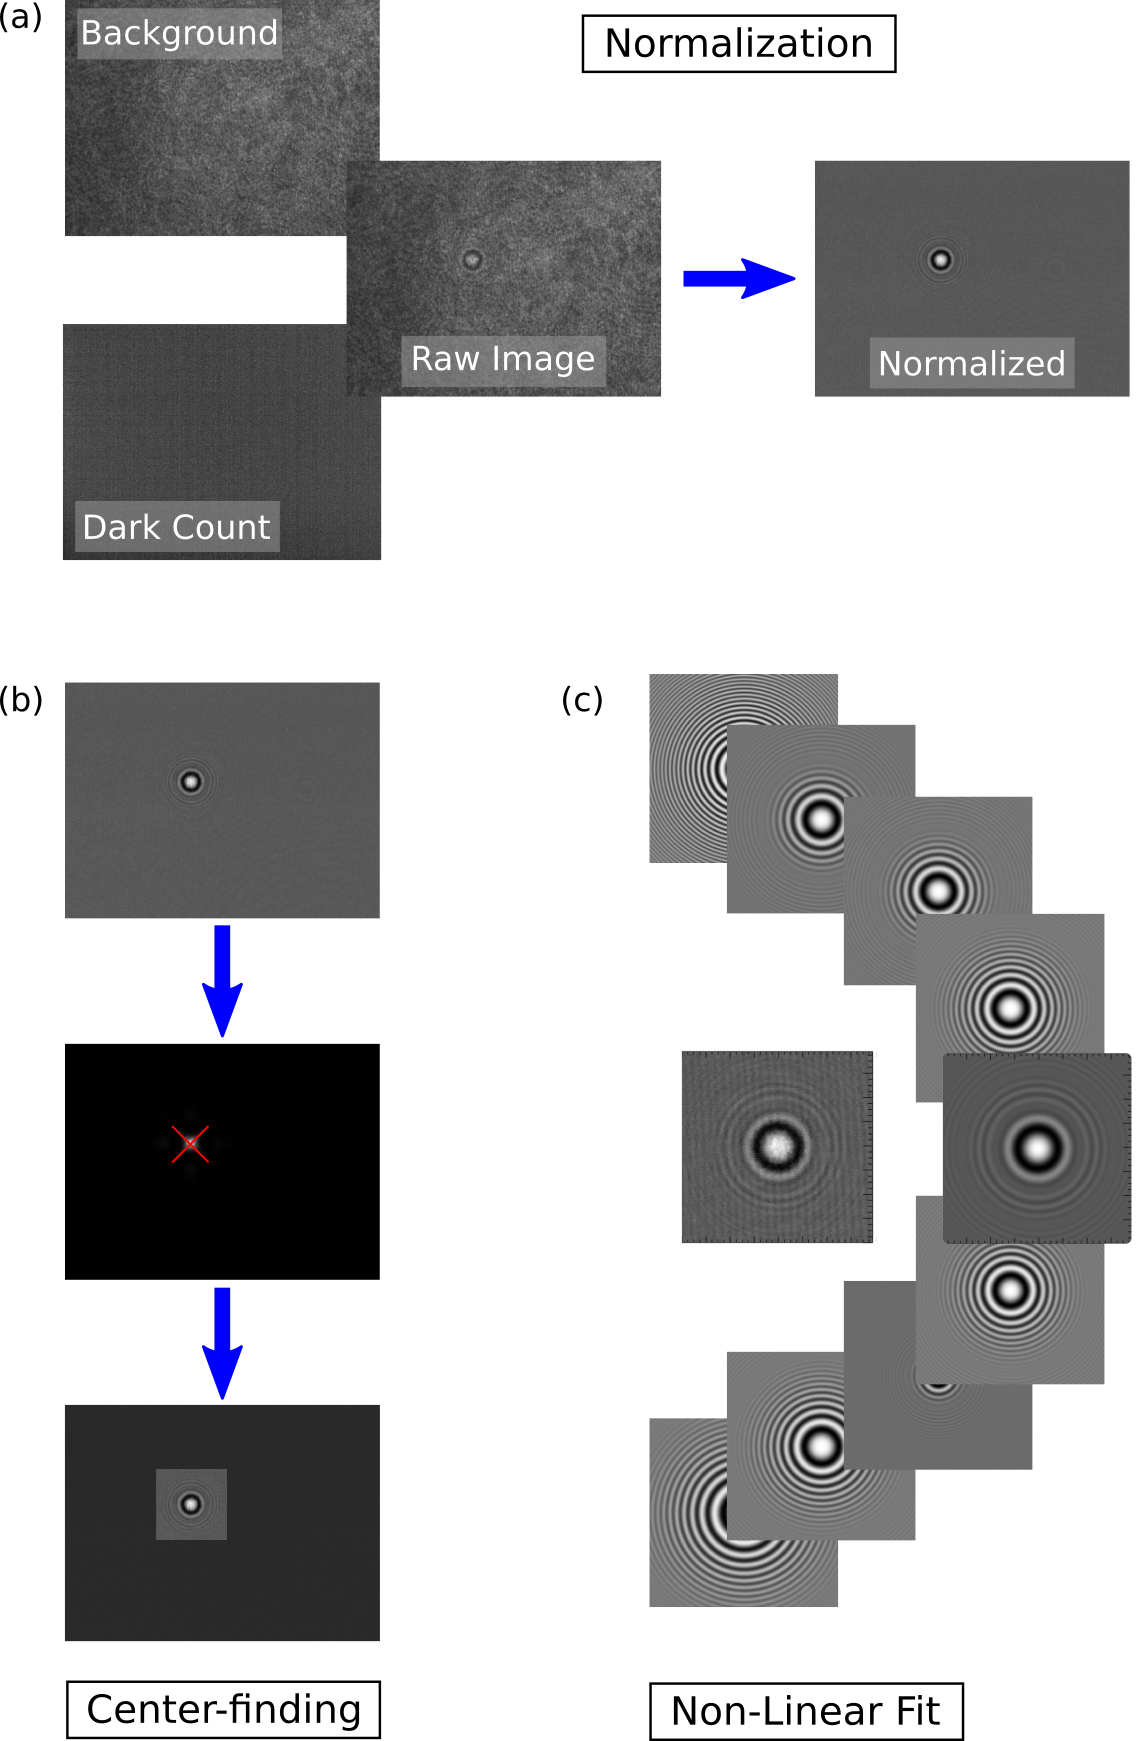
\includegraphics[width=0.8\textwidth]{hvm_image_analysis.png}
  \caption{(a) Raw image combines with the barkground and dark count
    images to produce a normalized frame. (b) Centroid finding on a transformed
    image reveals a holographic feature. (c) A cropped feature is compared
  against generated holograms to reveal the scatterer's properties.}
  \label{fig:image_analysis}
\end{figure}

The entire image analysis procedure is depicted in Fig.~\ref{fig:image_analysis}.
Image normalization is a necessary pre-processing step; Normalizing
the image eliminates the incident beam's magnitude $\abs{\einc}^2$
as a fitting parameter and mitigates contributions of additional
scatterers.
We therefore fit to a normalized image $b(x,y)$ as
\begin{align}
  b(x,y) &= \frac{ I(x,y) - I_d(x,y)}{ I_{bg}(x,y) - I_d(x,y)} 
\end{align}
where $I(x,y)$ is the image recorded by the camera,
$I_{bg}(x,y) = \abs{\einc(\vec{r})}^2$ is the background intensity,
and $I_d(x,y)$ is the dark count of the camera.
Fig.~\ref{fig:image_analysis}(a) demonstrates the effect of normalization.

The normalized image may or may not contain holographic features. If a feature
is detected,
our estimate of its center will serve as an initial estimate
for the in-plane position of the associated scatterer.
Feature detection and feature localization are the first two steps in analyzing
normalized holograms. A common heuristic is to coalesce the
extended holographic features into localized blobs and then to use a standard
centroid finding algorithm\cite{crocker96} on the transformed image. In this way,
the center of each blob will correspond to the center of a holographic feature.
Fig.~\ref{fig:image_analysis}(b)
summarizes this heuristic algorithm. An in-depth study of this algorithm, as well
as machine-learning alternatives will be presented in \autoref{ch:cascade}.

We fit each localized holographic feature to the Lorenz-Mie theory
with the Levenberg-Marquardt algorithm, otherwise known as damped least-squares.
The Levenberg-Marquardt algorithm interpolates between gradient descent which is a damped
first order algorithm, and the Gauss-Newton algorithm which is a second order
algorithm directed towards the nearest minimum. As with many fitting algorithms,
this method find a local minimum which may not be globally optimal. The fitting
procedure progressively finds model parameters that minimize the
chi-square metric for differences between the model and the experimental image.
The procedure terminates when one of three conditions is met:
\begin{enumerate}
\item the magnitude of the gradient drops below a threshold
\item the incremental change in chi-square drops below a predetermined threshold
\item a maximum number of iterations is exceeded.
\end{enumerate}
The final model parameters are interpreted as the actual parameters of the
scatterer. This procedure is repeated for every feature in every image.

\section{Best Practices}

Choices in instrumentation, sample preparation, and analysis may influence
the precision and accuracy of parameters through estimated the holographic
analysis. In this section, we outline considerations
and best practices for achieving optimal results by maximizing the
signal-to-noise ratio (SNR) of the image.

\subsection{Instrumentation}

Our inline holographic microscope is a compound microscope with
coherent illumination. It requires only a few pieces of equipment:
a coherent illumination source, an objective lens, a tube lens, and a digital
camera. The choice of components and their settings
determine the signal-to-noise ratio of each holographic feature.

The objective lens and tube lens are designed to magnify and relay the
intensity distribution in the focal plane to the camera.
The size of a pixel in the resulting image
must accordingly be calibrated. We use a calibrated reticle (Ted Pella 2280-13) to
gauge the size of a single pixel.%FIXME
The dynamic range and exposure period of the digital camera set lower and
upper bounds, respectively, for the intensity of the illumination.
To increase the signal-to-noise
ratio, it is desirable to maximize the intensity of the image without
saturating the camera. 

A high numerical aperture (NA) objective ensures that large-angle scattered
light contributes to the final image. Saglimbeni \emph{et al.}, for example,
were obliged to use a $\num{0.3}$ NA objective to track colloidal particles
trapped in a diamond anvil cell\cite{saglimbeni16}; as a result they found it necessary
to account for clipping of high spatial frequency in order to reasonably
fit each holographic feature. The NA 1.45 objective we used in our instrument
avoids such clipping.

\subsection{Sample Preparation}
\label{ssec:sample_prep}
Bright-field microscopy has a limited longitudinal resolution known as a
depth of focus. For magnifications of $\num{40}\times$ or higher, the depth
of focus is less than or equal to $\SI{1.0}{\um}$. With coherent
illumination, the longitudinal range is limited either by the
coherence length of the laser or by the signal-to-noise ratio of the
recorded intensity: in practice the longitudinal range far
exceeds the sample height. For this reason, HPC samples must be
diluted to ensure that not too many particles occupy the observation
volume. In our setup, the field of view
subtends a $\SI{80x65}{\um}$ area and a sealed sample
or flow cell has a depth of approximately $\SI{20}{\um}$. Therefore,
a sample number density of $\SI{E7}{\per\milli\liter}$ would correspond to
one scatterer in the field of view.

The long coherence length of the laser has another effect: every
smudge and defect in the optical train scatters light into the field of view. Cleaning
the glass surfaces can mitigate some of this unwanted scattering.
We chemically clean our microscope slides and cover slips
by immersing each in methanol and then isopropyl alcohol. Immediately
after the glass is dried by blowing nitrogen over the surface.
Normalization according to Eq.~\ref{eq:gen_norm} suppresses most of the remaining
unwanted interference features.

\section{Applications of Holographic Particle Characterization}

The utility of holographic particle characterization has been demonstrated by several groups
in a host of applications\cite{lee07a,fung12,saglimbeni16}. By simultaneously measuring the size, refractive index,
and three-dimensional position of individual scatters {\it in situ}, holographic
microscopy offers unparalleled insight into the composition of colloidal samples, as well
as the microscopic interactions that govern their behavior.

A sampling of just a few published studies illustrates the breadth of this technique's
applications.
Krishnatreya \emph{et al.} utilized the technique to measure Boltzmann's constant from the
size and three dimensional trajectory of a single sedimenting sphere \cite{krishnatreya14}.
Saglimbeni \emph{et al.} observed the compression of individual micrometer-sized
spheres
undergoing increased pressure in a diamond anvil cell\cite{saglimbeni16}. By using a sphere
of known size and refractive index, Shpaisman \emph{et al.} demonstrated HPC as an
approach for ``spatially resolved microrefractometry'' \cite{shpaisman12}.
Fung \emph{et al.} measured the three-dimensional diffusion tensor for
clusters of colloidal spheres with $\num{1}$\% precision and accuracy \cite{fung13}.

The utility of HPC extends beyond the academic domain as several commercial
applications have been established. Applications include assessing the quality of dairy
products \cite{cheong09a}, monitoring protein aggregation in biopharmaceuticals \cite{wang16}, detecting agglomeration in semiconductor polishing slurries \cite{cheong17}, 
and monitoring contaminants in wastewater \cite{philips17}.
%\cite{cheong17}, 
%Applications include
%
%
%
%performing microrheology \cite{cheong08}, 
%microrefractometry \cite{shpaisman12}, 
%and microporosimetry \cite{cheong11} measurements,
%assessing the quality of dairy products \cite{cheong09a},
%

%This technique has been demonstrated on both homogeneous
%and heterogeneous \cite{yevick14,philips17}
%dispersions of colloidal spheres, and has been extended to work for 
%colloidal clusters \cite{perry12,fung12,fung13}, and aggregates 
%\cite{wang16,wang16a}, as well as colloidal rods \cite{cheong10} 
%and other aspherical particles \cite{wang14using,hannel15}.
%
